%###############################################################
\section{Introduction}\label{sec:Intro}
%###############################################################

One of the exciting new directions of robotics is the design and development
of micro- and nanorobot systems, with the goal of letting a massive swarm of robots
perform complex operations in a complicated environment. Due to scaling 
issues, individual control of the involved robots becomes physically impossible:
while energy storage capacity drops with the third power of robot length,
medium resistance decreases much slower. As a consequence,
current micro- and nanorobot systems with many robots are steered and
directed by an external force that acts as a common control signal~\cite{Donald2013,Chiang2011,Hsi-Wen2012,Diller2013,Jing2013,Ou2013,Lanauze2013}.
These common control signals include global magnetic or electric fields,
chemical gradients, and turning a light source on and off.  

 \subsection{Selective Control with Global Inputs}
Having only one global signal that uniformly affects all robots at once
limits the swarm's ability to perform complex operations.
This control symmetry can be broken using interactions between the robot swarm
and obstacles in the environment. 
This paper builds on the techniques for controlling many simple particles with uniform control inputs presented in \cite{Becker2013f,Becker2014,Becker2014a}, where
we demonstrated how such a system could  implement digital computation.


\begin{figure}
\centering
\subfloat[]{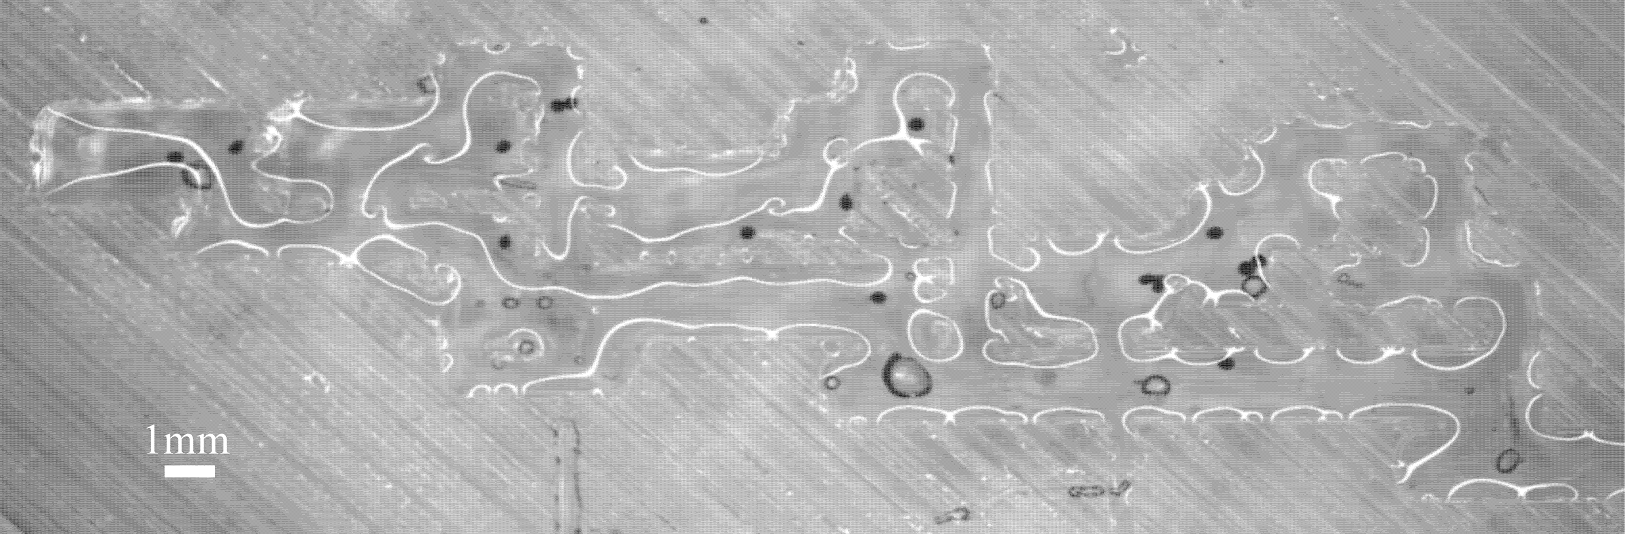
\includegraphics[width=3.1in]{Fig1.png}\label{fig:fig1a}} 
\newline
\subfloat[]{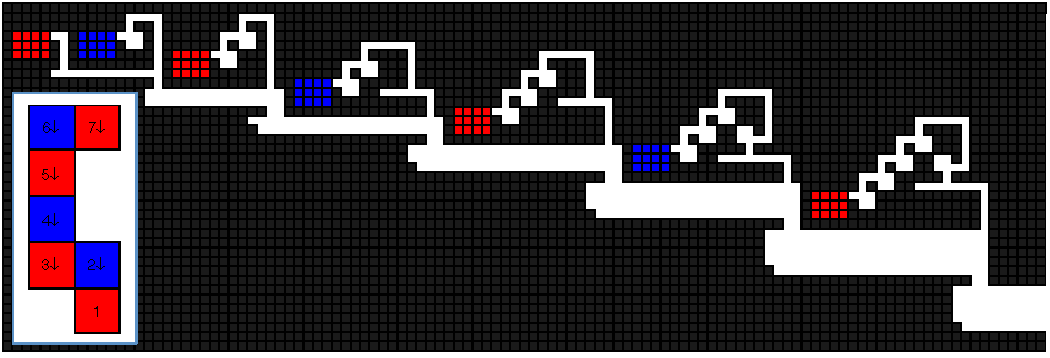
\includegraphics[width=3.1in]{fig1b2.pdf}\label{fig:fig1b}}
\caption{(a) 
Algorithm 4, as shown in the microscale. Alginate microrobots are shown throughout. Screenshot after move right command was executed. 
 (b) A seven tile factory. Each particle is actuated simultaneously by the same global field. The factory is designed so each clockwise control input assembles another component.}
\label{fig:1ab} 
\end{figure}



 \subsection{Model}\label{subsec:model}
Assume the following rules:
\begin{enumerate}
\item A planar  grid \emph{workspace} $W$ is filled with a number of unit-square robots (each occupying one cell of the grid)  and some fixed unit-square blocks.  Each unit square in the workspace is either  \emph{free}, which a particle may occupy or \emph{obstacle} which a robot may not occupy.  Each square in the grid can be referenced by its Cartesian coordinates $\bm{x}=(x,y)$.
\item All particles are commanded in unison: the valid commands are  ``Go Up" ($u$), ``Go Right" ($r$), ``Go Down" ($d$), or ``Go Left" ($l$).  
\item Particles all move until they 
	\begin{enumerate}
		\item hit an obstacle 
		\item hit a stationary particle. 
		\item share an edge with a compatible particle
	\end{enumerate}
	If a particle shares an edge with a compatible robot the two robots bond and from then on move as a unit.
A \emph{move sequence} $\bm{m}$ consists of an ordered sequence of moves $m_k$, where each $m_k\in\{u,d,r,l\}$  A representative move sequence is $\langle u,r,d,l,d,r,u,\ldots\rangle$. We assume the area of $W$ is finite and issue each command long enough for the robots to reach their maximum extent.
\end{enumerate}
